\rhead{Subsumption}

\chapter{Subsumption}
\label{sec:subsumption}

\begin{figure}[!h]
\centering
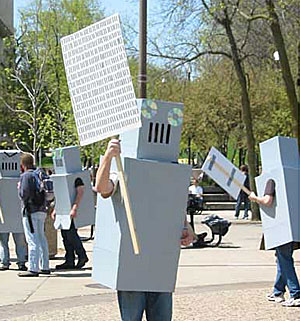
\includegraphics[width=0.8\columnwidth]{figures/9_robots.jpg}
\end{figure}

\newpage

\section{Introduction}

\noindent Your previous soccer-playing robots required some notion of state in order to function, such as robot pose, a map, ball location, etc.  State information, stored explicitly in variables, gave your controller a sense of context and immediate history about the robot's current situation.  Decision making at any moment in time is informed by state information in order to deliberate and plan into the future or take immediate action towards some future benefit.  State variables help our robots to be adaptive towards unexpected changes in the environment and flexible to new scenarios\footnote{Learning aims to provide a greater level of adaptability such that the robot has long-term context and history towards learning from experience.  It could roughly be thought of as never making the same mistake twice.}.  However, estimation of such variables comes at the cost of requiring greater computation, latency in decision making, and overall price tag for the robot.

Consider the case where you want to commercialize a soccer playing robot for a mass market\footnote{Because we are in Rhode Island, suppose you are making a robot for Hasbro.}.  Such a robot should not cost much money to purchase, on the order of the \$150 Roomba Red or \$250 Nintendo Wii.  Further, every additional component added to the robot, such as memory, processing, sensing, and actuators, increasingly cuts into your profit margin.  In such scenarios, reliance upon state variables costs you money\footnote{``Money'' in this case can be generalized to ``cost'' that limits practical implementation.  So, even if you are not fiscally motivated, such costs limit your ability realizing your technical visions.} and thus, you might be inclined to minimize the number of these variables.

Using reactive control, your robot controller in this assignment will rely upon no state variables and simply react to what can be sensed at the current instance of time.  In contrast to the deliberate intentionality of planning, reactive approaches rely upon {\bf emergent behavior} where the ``intelligence'' of the robot is both a factor of its decision making, the properties of the environment, and the dynamics of controller-environment interaction.  The Subsumption Architecture is one approach to reactive control that uses multiple robot controllers with a priority scheme.  In particular, each robot controller is capable of independently producing some robot behavior (such as wandering or obstacle avoidance) given certain applicability conditions (or preconditions) are met (such as whether an obstacle is present).  When their preconditions are met, higher priority controllers ``subsume''  lower priority controllers, whose decisions are then ignored.

\section{Key Concepts}

\begin{figure}[!h]
\centering
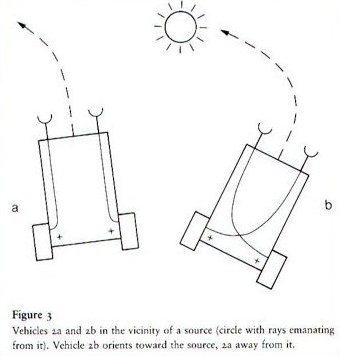
\includegraphics[width=0.5\columnwidth]{figures/9_embodied_intel.jpg}
\caption{Braitenberg vehicle}
\end{figure}

\begin{figure}[!h]
\centering
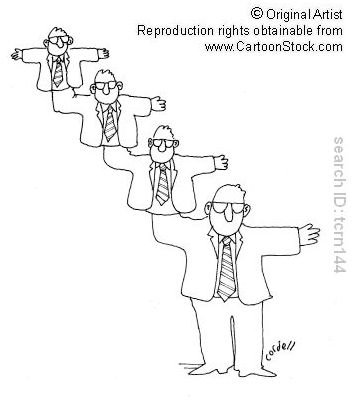
\includegraphics[width=0.5\columnwidth]{figures/9_hierarchy.jpg}
\caption{Subsumption-like hierarchy}
\end{figure}

\begin{figure}[!h]
\centering
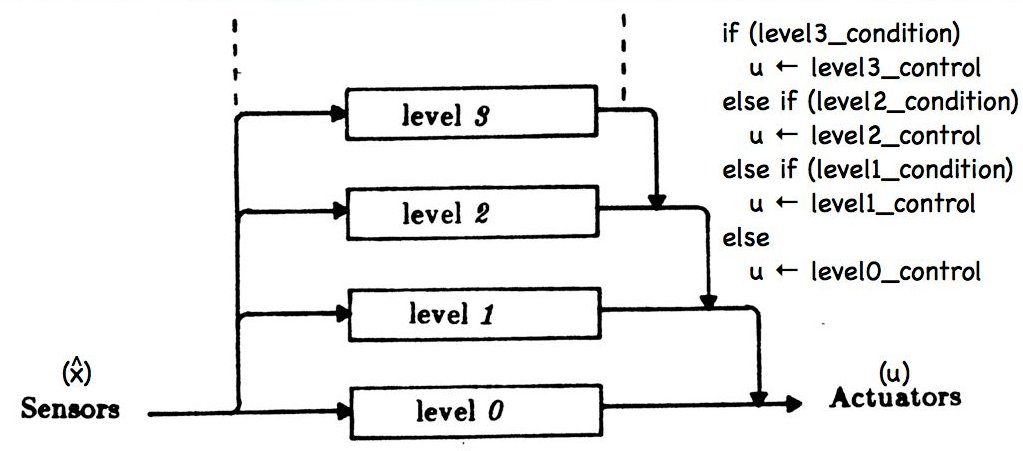
\includegraphics[width=0.8\columnwidth]{figures/9_sub1.jpg}
\caption{Implementing Subsumption}
\end{figure}

\begin{figure}[!h]
\centering
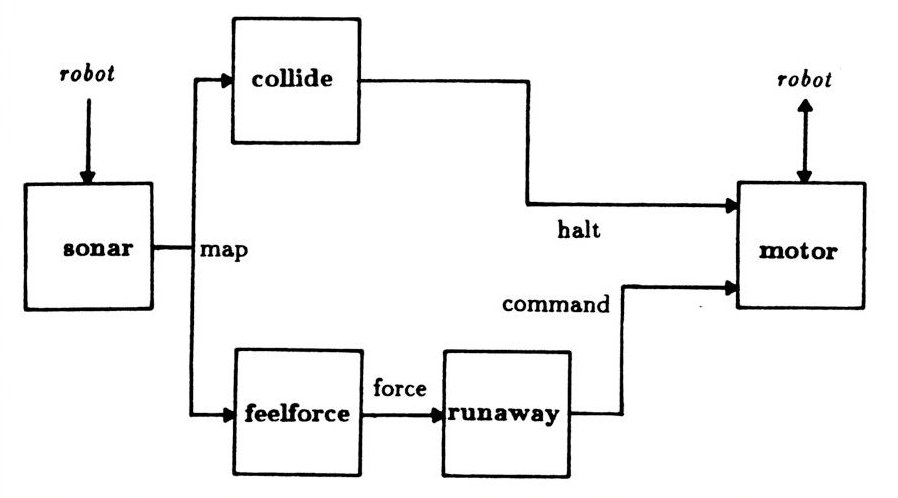
\includegraphics[width=0.7\columnwidth]{figures/9_sub2.jpg}
\caption{Subsumption Architecture 1}
\end{figure}

\begin{figure}[!h]
\centering
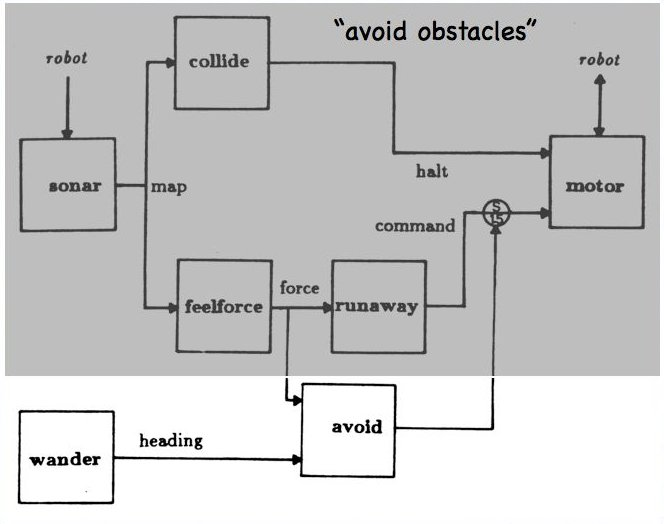
\includegraphics[width=0.6\columnwidth]{figures/9_sub3.jpg}
\caption{Subsumption Architecture 2}
\end{figure}

\begin{figure}[!h]
\centering
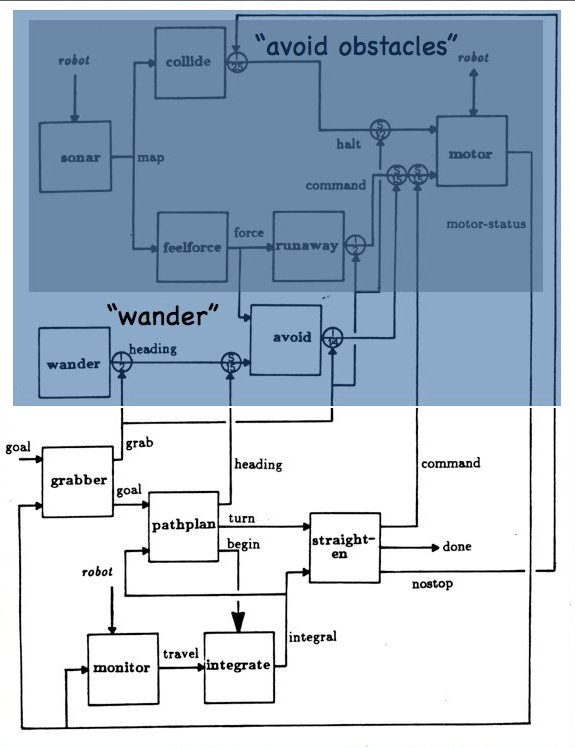
\includegraphics[width=0.5\columnwidth]{figures/9_sub4.jpg}
\caption{Subsumption Architecture 3}
\end{figure}

\subsection{Reactive Control}

\section{Project Infrastructure}

\begin{figure}
\centerline{
\mbox{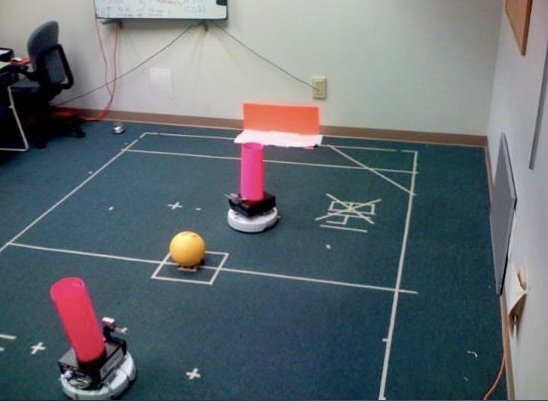
\includegraphics[width=3.00in]{figures/9_soccer1.jpg}}
\mbox{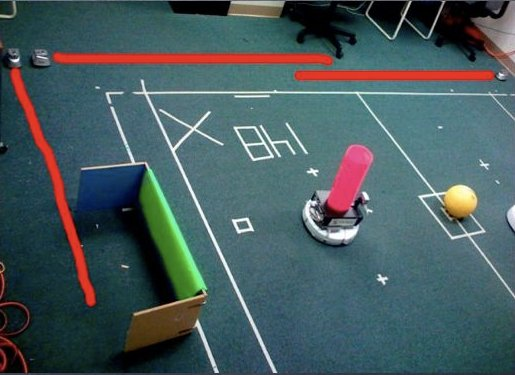
\includegraphics[width=3.00in]{figures/9_soccer2.jpg}}
}
\caption{Subsumption Soccer}
\end{figure}


\section{Instructions}

Develop a goal scoring controller without maintaining any state (history or timing variables).

In the current assignment, you will implement a robot soccer controller that uses only the robot's on-board immediate sensing and perception.  Specifically, you are only allowed to use the information provided in the {\bf current time instant} by Player's bumper, ir, and blobfinding proxies.  Timers, odometry, and variables that require history are not allowed in your client.  With this information, you are tasked with implementing a Subsumption architecture.  Towards this end, you must:

\begin{enumerate}
\item determine and implement an appropriate set of control behaviors for soccer
\item apply appropriate preconditions for each control behavior
\item determine and implement a priority scheme to coordinate the behaviors
\end{enumerate}

%\begin{figure}
\begin{wrapfigure}{r}{.55\columnwidth}[!ht]
\centering
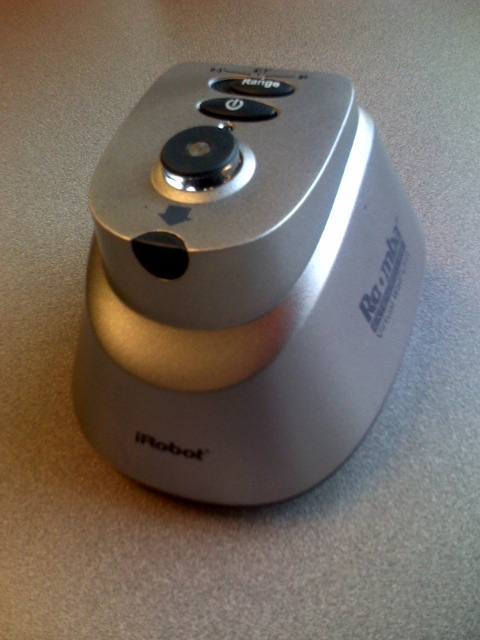
\includegraphics[width=0.4\textwidth]{figures/9_virtual_wall.jpg}
\caption{An iRobot Virtual Wall device emits an IR signal that can be received by the SmURV and provided to your client by Player's IR proxy.}
\label{fig:virtual_wall}
\end{wrapfigure}
%\end{figure}

Your robot will need to stay within the general field of play as given by the physical walls of the Roomba Lab and virtual walls placed around the pitch.  Additionally, your robot should make reasonable attempts to avoid collisions with other robots, which will be marked with pink fiducials.  We will definitely call player pushing penalties for this assignment!

Virtual walls (pictured to the right) are devices that emit infrared (IR) light that can be received by the iRobot Create and Roomba platforms.  The distribution of space covered by the emitted IR forms a beam that can extend over 8 feet.  These beams form an invisible barrier around the field that your robot should respect.  Your control client will have access to the SmURV's IR sensing through the IR proxy.

\subsection{Sensing a Virtual Wall}
All you have to do to sense a virtual wall is to create an IR proxy/interface\footnote{See \url{http://playerstage.sourceforge.net/doc/Player-cvs/player/classPlayerCc_1_1IrProxy.html} for C++ clients} and access the boolean flag ``wall hit'' through a call to the function GetRange(5); the 5 indicates the index of the virtual wall sensor.

In order to actually receive IR information from your SmURV you need to configure the player server to provide IR data. This is done by adding a few characters to the player configuration file on the SmURV (which is located in \texttt{/mnt/hda1/rootcopy/home/rlab/projects/[blind]smurv/[blind]smurv.cfg}). In the section
\begin{verbatim}
driver
(
    name "create"
    provides ["position2d:0" "bumper:0" "ircom:0"]
    port "/dev/ttyS0"
    safe 0
    alwayson 1
)
\end{verbatim}
change the \texttt{provides} line to the following:
\begin{verbatim}
    provides ["position2d:0" "bumper:0" "ircom:0" "ir:0"]
\end{verbatim}
After restarting your SmURV (or copying the configuration file into the virtual file system manually) you should have access to the IR sensors.

\begin{figure}
\centering
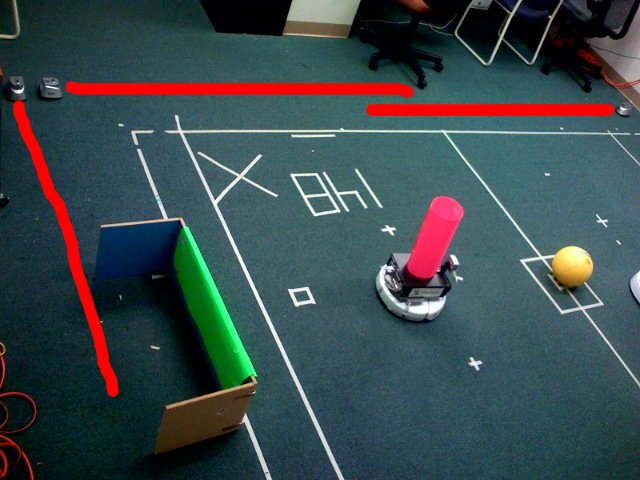
\includegraphics[width=0.7\textwidth]{figures/9_field1a.jpg}
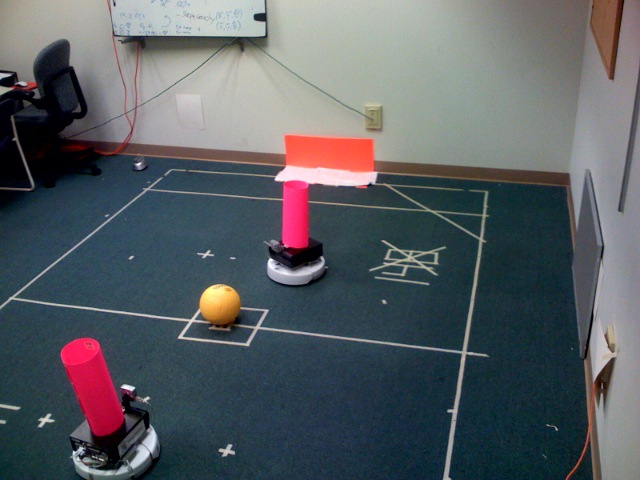
\includegraphics[width=0.6\textwidth]{figures/9_field2.jpg}
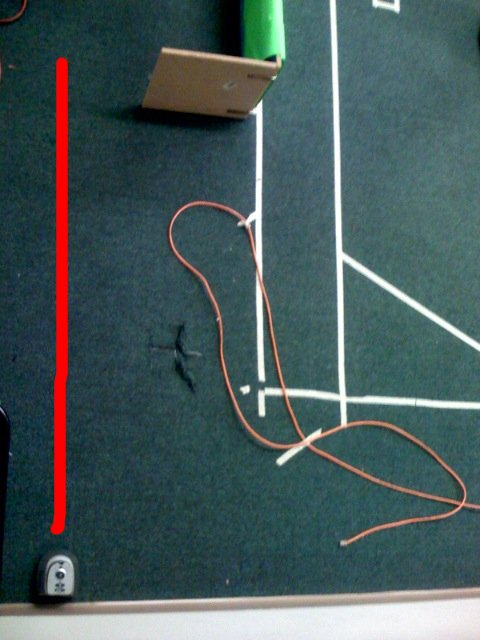
\includegraphics[width=0.34\textwidth]{figures/9_field3a.jpg}
\caption{Snapshot of the ``FC 148'' robot soccer field surrounded by virtual infrared (roughly marked in red) and real walls.  Your robot should properly react to both types of obstacles and other robots (with pink fiducials). }
\label{fig:field}
\end{figure}

\subsection{Behaviors and Prioritization}

You will be asked to demonstrate (either through a demo or in your report) that each control behavior functions independently and properly.  In addition, your independent behaviors will need to function together (without code modification) using a subsumption priority for coordination.  You will also be asked to randomly (based on the opinion of the course staff) reprioritize your behaviors to evaluate emergent behavior properties.

\section{Expected Outcomes and Reports}

\vspace{1cm}
\begin{tabular}{|l|l||l|l|}
\hline
{\large \bf Project Implementation} & \\
\hline
\hline
Individual Behaviors & 15\% \\
$\rightarrow$ Does each of your behaviors properly function? & \\
$\rightarrow$ Is each of your behaviors completely reactive, without state variables? & \\
$\rightarrow$ Do your control behaviors allow for modularity and transparent reprioritization? & \\
\hline
Behavior Choices & 15\% \\
$\rightarrow$ Do you have a sufficient set of behaviors for playing soccer? & \\
$\rightarrow$ Does your robot respect the environment (field of play) and avoid pushing other players? & \\
$\rightarrow$ Can your robot manipulate the ball and score goals? & \\
\hline
Subsumption Priority & 10\% \\
$\rightarrow$ Does your robot properly prioritize its individual control behaviors? & \\
$\rightarrow$ Does each of your behaviors have appropriate preconditions to allow for coordination? & \\
\hline
Soccer Proficiency & 5\% \\
$\rightarrow$ How well does your robot player soccer in the given environment? & \\
\hline
Controller Robustness & 5\% \\
$\rightarrow$ Does your controller run without interruption? & \\
\hline
\end{tabular}



\newpage
